\documentclass[11pt,a4paper,oneside,openany]{book}
\usepackage{fontspec}
\usepackage{xeCJK}
\setmainfont{Latin Modern Roman}
\setsansfont{Latin Modern Sans}
\setmonofont{Latin Modern Mono}[Scale=MatchLowercase]
\setCJKmainfont{FandolSong-Regular.otf}[BoldFont=FandolSong-Bold.otf,ItalicFont=FandolKai-Regular.otf]
\setCJKsansfont{FandolHei-Regular.otf}[BoldFont=FandolHei-Bold.otf]
\setCJKmonofont{FandolFang-Regular.otf}
\usepackage[a4paper,inner=23mm,outer=23mm,top=24mm,bottom=24mm,headheight=15pt]{geometry}
\usepackage{amsmath,amssymb,amsthm,bm,mathtools}
\usepackage{graphicx,booktabs,tabularx,array,longtable}
\usepackage{enumitem}
\usepackage{float}
\usepackage{xcolor}
\definecolor{CourseNavy}{HTML}{17324D}
\definecolor{CourseTeal}{HTML}{147D85}
\definecolor{CoursePale}{HTML}{F0F6F8}
\definecolor{CourseGray}{HTML}{536171}
\usepackage{titlesec}
\usepackage{setspace}
\setstretch{1.20}
\setlength{\parindent}{2em}
\setlength{\parskip}{0.25em}
\setlength{\emergencystretch}{2em}
\setlist{nosep,leftmargin=2em,topsep=0.4em}
\setlist[enumerate,1]{label=\arabic*.}
\usepackage[most]{tcolorbox}
\newtcolorbox{coursebox}[1]{enhanced,breakable,colback=CoursePale,colframe=CourseTeal,
  boxrule=0.45pt,arc=1mm,left=3mm,right=3mm,top=2mm,bottom=2mm,
  title={#1},fonttitle=\bfseries\sffamily,coltitle=white,
  before skip=1em,after skip=1em}
\titleformat{\chapter}[display]{\sffamily\bfseries\color{CourseNavy}\huge}
  {\large 第\thechapter 讲}{0.6em}{}
\titlespacing*{\chapter}{0pt}{-10pt}{20pt}
\titleformat{\section}{\Large\sffamily\bfseries\color{CourseNavy}}{\thesection}{0.6em}{}
\titleformat{\subsection}{\large\sffamily\bfseries\color{CourseTeal}}{\thesubsection}{0.6em}{}
\titleformat{\subsubsection}{\normalsize\sffamily\bfseries}{\thesubsubsection}{0.6em}{}
\setcounter{secnumdepth}{2}
\setcounter{tocdepth}{1}
\theoremstyle{definition}
\newtheorem{definition}{定义}[chapter]
\newtheorem{example}{例题}[chapter]
\newtheorem{exercise}{习题}[chapter]
\theoremstyle{plain}
\newtheorem{theorem}{定理}[chapter]
\newtheorem{proposition}[theorem]{命题}
\newtheorem{lemma}[theorem]{引理}
\newtheorem{corollary}[theorem]{推论}
\theoremstyle{remark}
\newtheorem{remark}{说明}[chapter]
\renewcommand{\proofname}{证明}
\newcommand{\R}{\mathbb R}
\newcommand{\E}{\mathbb E}
\DeclareMathOperator{\Var}{Var}
\DeclareMathOperator{\Cov}{Cov}
\DeclareMathOperator{\diag}{diag}
\DeclareMathOperator{\tr}{tr}
\DeclareMathOperator{\rank}{rank}
\DeclareMathOperator*{\argmin}{arg\,min}
\DeclareMathOperator*{\argmax}{arg\,max}
\newcommand{\norm}[1]{\left\lVert#1\right\rVert}
\newcommand{\inner}[2]{\left\langle#1,#2\right\rangle}
\usepackage[numbers,sort&compress]{natbib}
\usepackage{url}
\usepackage[unicode,colorlinks=true,linkcolor=CourseNavy,citecolor=CourseTeal,urlcolor=CourseTeal,
  bookmarksnumbered=true,pdfauthor={冯恺睿},pdftitle={凸优化与非线性优化：2027讲义}]{hyperref}
\usepackage{bookmark}
\usepackage{fancyhdr}
\pagestyle{fancy}
\fancyhf{}
\fancyhead[L]{\small\sffamily\color{CourseGray}凸优化与非线性优化}
\fancyhead[R]{\small\sffamily\color{CourseGray}2027 讲义}
\fancyfoot[C]{\small\thepage}
\renewcommand{\headrulewidth}{0.3pt}
\fancypagestyle{plain}{\fancyhf{}\fancyfoot[C]{\small\thepage}\renewcommand{\headrulewidth}{0pt}}
\renewcommand{\contentsname}{目录}
\renewcommand{\bibname}{参考文献}
\renewcommand{\figurename}{图}
\renewcommand{\tablename}{表}
\newcommand{\coursecover}[3]{%
  \hypersetup{pageanchor=false}
  \begin{titlepage}
  \setlength{\parindent}{0pt}
  \thispagestyle{empty}
  \vspace*{15mm}
  {\sffamily\color{CourseTeal}\Large 2027 \quad COURSE NOTES\par}
  \vspace{12mm}
  {\sffamily\bfseries\color{CourseNavy}\fontsize{31}{42}\selectfont 凸优化与\\非线性优化\par}
  \vspace{7mm}
  {\sffamily\color{CourseGray}\Large Convex and Nonlinear Optimization\par}
  \vspace{13mm}
  {\color{CourseTeal}\rule{\textwidth}{1.1pt}\par}
  \vspace{8mm}
  {\sffamily\bfseries\color{CourseNavy}\LARGE #1\par}
  \vspace{6mm}
  {\large #2\par}
  \vspace{12mm}
  {\normalsize #3\par}
  \vfill
  {\large 主讲：冯恺睿\par}
  \vspace{3mm}
  {\small 同济大学／上海创智学院课程材料\par}
  \vspace{5mm}
  {\small\color{CourseGray}从最优性条件、下降方法与随机噪声，到神经网络的更新几何与参数化。\par}
  \end{titlepage}
  \hypersetup{pageanchor=true}
}

\begin{document}
\coursecover{第2讲：对偶、KKT与约束优化}{3学时理论}{用可行性、乘子与互补松弛刻画约束问题，并连接投影、近端与增广Lagrangian算法。}
\tableofcontents
\setcounter{chapter}{1}
\chapter{对偶、KKT 与约束优化}
\label{l2:chapter}

\begin{coursebox}{本讲目标与课堂安排}
无约束问题在最优点满足 $\nabla f=0$；加入预算、守恒或安全约束后，最优点常在边界，梯度可以不为零。本讲的核心是用对偶与 Karush--Kuhn--Tucker（KKT）条件描述这种边界最优性，并据此构造可计算的算法。

本讲为三个理论学时。按每学时45分钟，建议安排：对偶与 Slater 条件30分钟，KKT 的条件边界及两个二维例题55分钟，投影与近端25分钟，罚函数与增广 Lagrangian 25分钟。LICQ 必要性证明、完整近端收敛证明和对偶迭代的补充例子为选读。课堂结束时，应能独立列出并核验完整 KKT 条件，解释乘子的符号与尺度，并说明凸问题的最优证书和非凸问题的驻点证据有何不同。
\end{coursebox}

\section{约束改变了最优性的表达}
\label{l2:problem}

本讲采用统一符号
\begin{equation}
 \begin{aligned}
 \min_{x\in\R^d}\quad & f(x),\\
 \text{s.t.}\quad & g_i(x)\leq0,\qquad i=1,\ldots,m,\\
 & h_j(x)=0,\qquad j=1,\ldots,p.
 \end{aligned}
 \label{l2:primal}
\end{equation}
除另行说明外，$f,g_i,h_j$ 均连续可微。可行点满足所有约束，可行集合记为 $C$，原始最优值记为 $p^*$。在点 $x\in C$，满足 $g_i(x)=0$ 的不等式称为活跃约束，其指标集合为 $\mathcal I(x)$。严格满足 $g_i(x)<0$ 的约束在足够小的邻域内不限制位移方向。

例如，$\min_{x\geq0}x$ 的唯一最优点是0，但目标导数是1而不是0。向负方向移动可以减少目标，却违反约束；向正方向移动虽然可行，却增加目标。因此约束最优性要求的是“没有可行下降方向”，而非“所有方向的一阶变化都为零”。

\begin{definition}[本讲采用的凸规划形式]
当 $f$ 与所有 $g_i$ 是凸函数，且等式约束为仿射形式 $h(x)=Ax-b$ 时，称\eqref{l2:primal}为凸规划。它的可行集合是凸集。等式若写成一般非线性凸函数等于0，其零水平集也未必凸，不能只凭“每个函数都凸”就认定整个问题是凸规划。
\end{definition}

约束表示本身也有影响。例如 $x=0$ 与 $x^2\leq0$ 定义同一个集合，但它们在0处的约束梯度分别为1和0。算法和乘子条件需要使用约束函数的导数，所以仅知道可行集合相同，还不足以保证两种表示同样适合数值求解。

\section{Lagrangian 与对偶：先建立下界}
\label{l2:duality}

\subsection{为什么不等式乘子必须非负}

引入不等式乘子 $\lambda\in\R^m$ 与等式乘子 $\nu\in\R^p$，定义 Lagrangian
\begin{equation}
 \mathcal L(x,\lambda,\nu)
 =f(x)+\sum_{i=1}^m\lambda_i g_i(x)
       +\sum_{j=1}^p\nu_jh_j(x).
 \label{l2:lagrangian}
\end{equation}
当 $x$ 可行且 $\lambda\geq0$ 时，$\lambda_i g_i(x)\leq0$，而等式项为0，故 $\mathcal L(x,\lambda,\nu)\leq f(x)$。乘子的符号由这一不等式决定；若把原约束改写为 $g_i(x)\geq0$，就必须相应调整符号约定。等式乘子没有符号限制。

定义对偶函数
\begin{equation}
 q(\lambda,\nu)=\inf_{x\in\R^d}\mathcal L(x,\lambda,\nu),
 \label{l2:dual-function}
\end{equation}
它允许取 $-\infty$。这里对 $x$ 的最小化已经去掉原约束，因为约束信息进入了乘子项。若误把 $\inf_x$ 再限制在原可行集合，会得到另一个对象，通常失去对偶方法的作用。

\begin{proposition}[弱对偶]
\label{l2:prop-weak-duality}
对任意原始可行点 $x$ 和任意 $\lambda\geq0,\nu$，均有
\[
 q(\lambda,\nu)\leq\mathcal L(x,\lambda,\nu)\leq f(x).
\]
因此对偶问题
\begin{equation}
 d^*=\sup_{\lambda\geq0,\nu}q(\lambda,\nu)
 \label{l2:dual-problem}
\end{equation}
满足 $d^*\leq p^*$。这个结论不要求原问题凸。
\end{proposition}

对每个固定 $x$，$\mathcal L$ 关于 $(\lambda,\nu)$ 都是仿射函数。仿射函数族的逐点下确界是凹函数，所以 $q$ 总是凹的，即使原问题非凸。对偶问题是在凸集合 $\lambda\geq0$ 上最大化凹函数；“对偶问题具有凸优化结构”并不意味着原问题的非凸性已经消失，因为可能存在正的对偶间隙 $p^*-d^*$。

\subsection{可计算的最优性证书}

若 $x$ 原始可行、$(\lambda,\nu)$ 对偶可行，且 $q$ 有限，则
\begin{equation}
 0\leq f(x)-p^*\leq f(x)-q(\lambda,\nu).
 \label{l2:gap-certificate}
\end{equation}
因此，一个可行解与一个下界可以共同构成最优性证书。优化软件报告的 primal--dual gap 正是利用这一思想。若当前 $x$ 不可行，$f(x)$ 不能直接作为可行最优值的上界，此时即使数值上的“gap”很小，也不能使用\eqref{l2:gap-certificate}。

对偶值与乘子并不是随意添加的辅助变量。它们分别提供“目前至少不可能比什么值更好”和“哪些约束正在阻止目标进一步下降”的信息。后者会在影子价格分析中变得具体。

\section{强对偶与 Slater 条件}
\label{l2:slater}

弱对偶始终成立，强对偶 $d^*=p^*$ 则需要额外条件。本讲使用一个足够常用、假设清楚的版本\citep{Boyd2004}。

\begin{theorem}[Slater 条件下的强对偶]
\label{l2:thm-slater}
设 $f,g_1,\ldots,g_m$ 在整个 $\R^d$ 上有限、凸且可微，$h(x)=Ax-b$。假设最优值有限，并存在严格可行点 $\bar x$ 满足
\[
 A\bar x=b,\qquad g_i(\bar x)<0\quad(i=1,\ldots,m).
\]
则 $d^*=p^*$，且存在达到对偶最优值的乘子 $(\lambda^*,\nu^*)$。若原始最优值也在某个 $x^*$ 处取到，则该点存在满足完整 KKT 条件的乘子。
\end{theorem}

这里的严格可行只针对不等式；等式必须精确满足，不能要求“严格等于”。当模型具有受限定义域时，还要使用相对内部来表达合适的 Slater 条件。本讲把函数设为在整个 $\R^d$ 上有限，是为了避免在初次学习时把域的边界和不等式约束混在一起。

Slater 是充分条件，不是必要条件。某个问题不满足它，不能立即宣布存在对偶间隙；可能仍然强对偶，也可能最优乘子不取到。应分别检查“最优值是否相等”和“最优解或乘子是否存在”。下一节的退化约束例子会同时说明这些区别。

\paragraph{选读：强对偶证明的几何入口.}
把约束右端放宽为 $g(x)\leq u$、$h(x)=v$，考察集合
\[
 \mathcal A=\{(u,v,t):\ \exists x,\quad
       g(x)\leq u,\ h(x)=v,\ f(x)\leq t\}.
\]
目标与不等式的凸性、等式的仿射性使 $\mathcal A$ 为凸集，分离超平面可以为最优值提供线性下界。若等式存在冗余，应先删除冗余等式，或在可达扰动的相对仿射空间中使用分离定理；否则可能存在仅来自不可达等式扰动方向的退化法向量。作此处理后，严格可行排除相关的不正常分离情形，使目标系数能够规范化为1。将规范化后的约束系数写成 $\lambda\geq0,\nu$，便得到达到 $p^*$ 的 Lagrangian 下界。这是 Slater 条件与乘子存在之间的联系；完整分离论证可阅读\citet{Boyd2004}的对偶章节。

\section{KKT 条件：四组方程和三种适用范围}
\label{l2:kkt}

\subsection{完整条件不能只剩“梯度为零”}

对候选点 $(x^*,\lambda^*,\nu^*)$，完整 KKT 条件是
\begin{align}
 g_i(x^*)&\leq0,\quad h_j(x^*)=0
 &&\text{（原始可行性）},\label{l2:kkt-primal}\\
 \lambda_i^*&\geq0
 &&\text{（对偶可行性）},\label{l2:kkt-dual}\\
 \lambda_i^*g_i(x^*)&=0
 &&\text{（互补松弛）},\label{l2:kkt-complementarity}\\
 \nabla f(x^*)+\sum_i\lambda_i^*\nabla g_i(x^*)
       +\sum_j\nu_j^*\nabla h_j(x^*)&=0
 &&\text{（驻点条件）}.
 \label{l2:kkt-stationarity}
\end{align}
互补松弛的含义是：严格松弛约束的乘子必须为0；乘子为正的约束必须活跃。反向命题不成立，活跃约束的乘子也可以为0。列出驻点方程而忘掉乘子的非负性，会把不可接受的候选点混入解集。

\begin{theorem}[凸问题中 KKT 的充分性与必要性]
\label{l2:thm-convex-kkt}
设 $f,g_i$ 凸且可微，$h$ 仿射。
\begin{enumerate}
 \item 只要某个三元组满足全部 KKT 条件，$x^*$ 就是全局最优点，乘子为对偶最优解，且对偶间隙为0。此充分性不需要额外的 Slater 条件。
 \item 若最优点存在，且满足定理\ref{l2:thm-slater}的 Slater 假设，则每个原始最优点均存在使 KKT 成立的乘子。
\end{enumerate}
\end{theorem}

\begin{proof}
先证充分性。因为 $\lambda^*\geq0$，$x\mapsto\mathcal L(x,\lambda^*,\nu^*)$ 是凸函数。驻点条件使 $x^*$ 为它的全局极小点，互补松弛和可行性给出 $\mathcal L(x^*,\lambda^*,\nu^*)=f(x^*)$。对任意可行 $x$，
\[
 f(x)\geq\mathcal L(x,\lambda^*,\nu^*)
 \geq\mathcal L(x^*,\lambda^*,\nu^*)=f(x^*).
\]
同时 $q(\lambda^*,\nu^*)=f(x^*)$，所以乘子也达到对偶最优值。

再证必要性。Slater 保证存在对偶最优乘子，且 $q(\lambda^*,\nu^*)=f(x^*)$。弱对偶中的两个不等式此时必须都取等号：$x^*$ 最小化 Lagrangian，所以其梯度为0；又因为每个 $\lambda_i^*g_i(x^*)\leq0$ 而总和为0，每一项都必须为0，得到互补松弛。
\end{proof}

\subsection{非凸问题中的必要性：约束资格条件}

\begin{definition}[线性无关约束资格条件 LICQ]
在可行点 $x^*$，如果向量集合
\[
 \{\nabla g_i(x^*):i\in\mathcal I(x^*)\}
 \ \cup\ \{\nabla h_j(x^*):j=1,\ldots,p\}
\]
线性无关，则称 LICQ 在该点成立。只把活跃不等式放入这个集合。
\end{definition}

\begin{theorem}[非凸局部最优点的 KKT 必要条件]
\label{l2:thm-licq}
设目标与约束在 $x^*$ 邻域连续可微，$x^*$ 是局部极小点，且 LICQ 成立。则存在满足 KKT 条件的乘子，且这些乘子唯一。该定理不要求凸性，也不保证任何 KKT 点是局部或全局极小点。
\end{theorem}

\paragraph{选读：必要性证明.}
考虑线性化可行方向 $d$，满足 $\nabla h_j(x^*)^\top d=0$、$\nabla g_i(x^*)^\top d\leq0$ 对所有活跃 $i$ 成立。若同时 $\nabla f(x^*)^\top d<0$，LICQ 允许找到方向 $d_0$，使所有等式的一阶变化为0、所有活跃不等式的一阶变化为 $-1$。对足够小的 $\epsilon>0$，$d+\epsilon d_0$ 仍为下降方向，而且严格进入所有活跃不等式内部。等式 Jacobian 满秩，隐函数定理给出具有这一切向量的等式可行曲线；足够短的一段曲线便是可行下降路径，与局部最优矛盾。

因此不存在上述线性化下降方向。有限维 Farkas 择一定理表明，这等价于 $-\nabla f(x^*)$ 属于活跃约束梯度的非负锥与等式梯度线性空间之和。这恰好给出驻点条件中的非负 $\lambda$ 与自由 $\nu$；非活跃乘子置0后得到互补松弛。最后，若有两组乘子，减去两条驻点方程，LICQ 强制它们完全相同。相关约束资格与必要条件可参见\citet{Nocedal2006}。

\begin{example}[LICQ 失败：有最优解但不存在 KKT 乘子]
\label{l2:ex-licq-failure}
考虑凸问题
\[
 \min_x x\qquad\text{s.t.}\qquad x^2\leq0.
\]
唯一可行点是 $x^*=0$，因此它当然全局最优。可是 $g'(0)=0$，LICQ 失败，驻点方程要求 $1+\lambda\cdot0=0$，没有任何有限乘子能够满足。

这个例子还可以完整算出对偶。当 $\lambda>0$，
\[
 q(\lambda)=\inf_x(x+\lambda x^2)=-\frac1{4\lambda};
\]
当 $\lambda=0$，$q(0)=-\infty$。故 $d^*=\sup_{\lambda\geq0}q(\lambda)=0=p^*$，但对偶最优值只在 $\lambda\to\infty$ 时逼近，没有有限最优乘子。这里强对偶成立，Slater 不成立，KKT 乘子不存在，三个事实并不矛盾。

若把同一集合写为等式 $h(x)=x=0$，驻点条件成为 $1+\nu=0$，可取 $\nu=-1$。改变约束表示修复了导数退化，而没有改变可行点。
\end{example}

LICQ 失败并不意味着 KKT 一定失败。例如 $\min_x\tfrac12(x-1)^2$，约束为 $x\leq0$ 与 $2x\leq0$。在最优点0，两条活跃梯度相关，但严格可行点 $x=-1$ 存在。KKT 乘子满足 $\lambda_1+2\lambda_2=1$、$\lambda\geq0$，有无穷多组。这说明 Slater 关注凸对偶与乘子存在，LICQ 还排除了活跃约束的冗余并保证乘子唯一；不能把二者当作同一个条件。

\subsection{KKT 点为什么未必是非凸极小点}

考虑 $\min_{-1\leq x\leq1}-x^2$。在 $x=0$，两条不等式均不活跃，取乘子全为0便满足 KKT；但该点是严格局部极大点，真正的最优点为 $\pm1$。因此，在非凸问题中求解 KKT 方程通常只是在找候选点。

二阶判断还必须沿可行方向进行。对于仅含等式的二阶可微问题，在 LICQ 与 KKT 成立时，局部极小点要求 Lagrangian Hessian 在切空间 $\{d:J_h(x^*)d=0\}$ 上半正定；若在所有非零切向量上正定，则可获得严格局部极小的充分条件。带不等式时，应进一步使用临界锥，不能直接要求或检查整个空间上的 Hessian 正定来替代约束二阶分析。

\begin{coursebox}{使用 KKT 前先辨认问题属于哪一类}
凸目标、凸不等式、仿射等式：满足 KKT 就是全局最优证书；要保证最优点一定有乘子，可以检查 Slater。一般非凸问题：局部最优点在 LICQ 等约束资格下必须满足 KKT；找到 KKT 点之后仍需二阶条件、问题结构或其他证据判断其性质。退化约束：最优点可能没有有限 KKT 乘子，应先检查约束表示和资格条件。
\end{coursebox}

\section{完整例题：二维二次规划与影子价格}
\label{l2:worked}

\subsection{预算约束下的投影问题}

\begin{example}[从活跃集到原始--对偶证书]
\label{l2:ex-budget}
给定预算 $b>0$，求解
\begin{equation}
 \min_{x_1,x_2}\ \frac12\bigl[(x_1-2)^2+(x_2-1)^2\bigr],
 \quad x_1+x_2\leq b,\quad x_1\geq0,\ x_2\geq0.
 \label{l2:budget-problem}
\end{equation}
这是把点 $(2,1)$ 投影到非负预算集合。令预算乘子为 $\lambda\geq0$，非负约束 $-x_i\leq0$ 的乘子为 $\alpha_i\geq0$。Lagrangian 为
\[
 \mathcal L=\frac12\norm{x-(2,1)^\top}^2
        +\lambda(x_1+x_2-b)-\alpha_1x_1-\alpha_2x_2.
\]
驻点条件是
\[
 x_1-2+\lambda-\alpha_1=0,\qquad
 x_2-1+\lambda-\alpha_2=0.
\]
还需同时满足三条可行性、三个非负乘子条件，以及
\[
 \lambda(x_1+x_2-b)=0,\qquad\alpha_1x_1=\alpha_2x_2=0.
\]

先取 $b=2$。无约束解 $(2,1)$ 不可行，因此尝试预算活跃、两坐标均为正。互补松弛给出 $\alpha_1=\alpha_2=0$，于是 $x_1=2-\lambda$、$x_2=1-\lambda$。结合 $x_1+x_2=2$，得
\[
 x^*=(3/2,1/2)^\top,\qquad\lambda^*=1/2,
 \qquad\alpha^*=0.
\]
解出的坐标确实为正，乘子也非负，所以所猜活跃集自洽。问题凸，因此这已经证明全局最优；强凸目标进一步保证该原始解唯一。

还可以计算独立的对偶下界。令 $c=(\lambda-\alpha_1,\lambda-\alpha_2)^\top$，对 $x$ 无约束最小化得到
\[
 q(\lambda,\alpha)
 =3\lambda-2\alpha_1-\alpha_2
 -\frac12\bigl[(\lambda-\alpha_1)^2+(\lambda-\alpha_2)^2\bigr]
 -\lambda b.
\]
在上述乘子处 $q=1/4$；原始目标也是 $1/4$，所以 gap 精确为0。

现在让 $b$ 变化。对 $0<b\leq1$，第二坐标被压到0，得到 $x^*=(b,0)^\top$、$\lambda^*=2-b$、$\alpha_2^*=1-b$、$\alpha_1^*=0$。对 $1\leq b\leq3$，两个坐标非负，解为 $((b+1)/2,(b-1)/2)^\top$，预算乘子为 $(3-b)/2$。当 $b\geq3$，无约束解已经可行，所有乘子可以取0。最优值为
\begin{equation}
 p(b)=
 \begin{cases}
 \tfrac12[(b-2)^2+1],&0<b\leq1,\\
 (3-b)^2/4,&1\leq b\leq3,\\
 0,&b\geq3.
 \end{cases}
 \label{l2:budget-value}
\end{equation}
各区间都满足 $p'(b)=-\lambda^*(b)$。例如在 $b=2$，多增加很小的预算 $\delta b$，最优目标约下降 $\delta b/2$。在 $b=3$，预算约束活跃但乘子为0，这是“活跃不一定正乘子”的具体例子。
\end{example}

\begin{figure}[htbp]
\centering
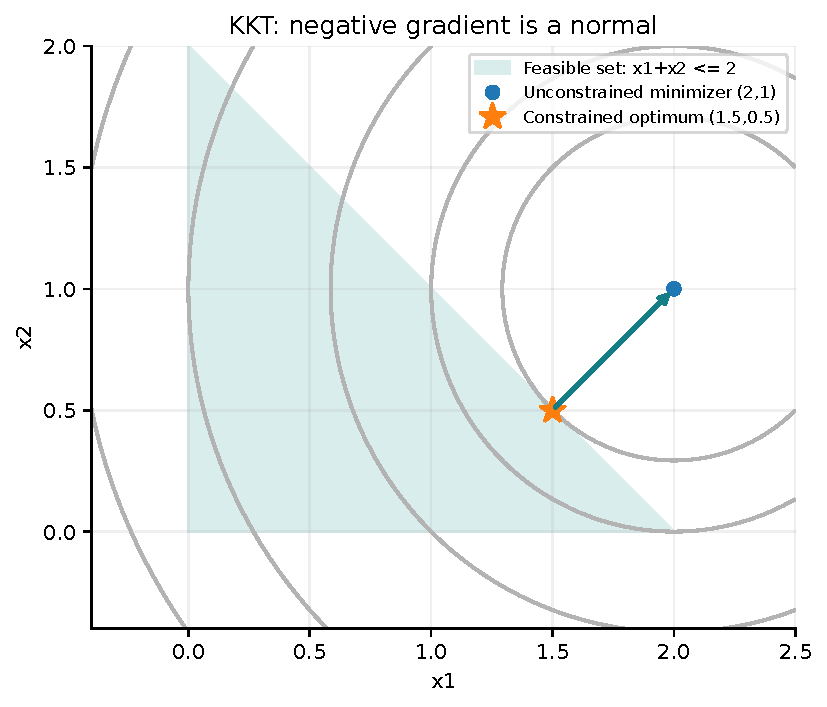
\includegraphics[width=0.85\textwidth]{figures/kkt_geometry.pdf}
\caption{预算为 $b=2$ 时，将 $z=(2,1)^\top$ 投影到可行集 $\{x\geq0:x_1+x_2\leq2\}$。最优点为 $x^*=(1.5,0.5)^\top$，预算约束活跃而两个非负约束均不活跃。预算边界的外法向量为 $(1,1)^\top$，乘子 $\lambda^*=0.5$ 使 $x^*-z+\lambda^*(1,1)^\top=0$；投影位移与活跃边界正交。目标值与对偶下界均为 $1/4$，给出零间隙的全局最优证书。}
\label{l2:fig-kkt-geometry}
\end{figure}

这个例子展示了一种可复用的解题顺序：先写标准符号，再猜活跃集，用互补松弛删去无关乘子，解驻点与活跃约束方程，最后回代核验全部不等式。若核验失败，改变活跃集；不能只保留代数方程的解。

\subsection{球约束也是二次约束：乘子的单位必须明确}

\begin{example}[二次目标与二次约束的完整 KKT 解]
\label{l2:ex-ball}
求解
\[
 \min_{x\in\R^2}\frac12\norm{x-z}^2,
 \qquad \norm x^2\leq4,\qquad z=(3,4)^\top.
\]
目标强凸，约束凸，严格可行点为0。由于 $\norm z=5>2$，无约束解不可行，最优点位于球面。写出
\[
 \mathcal L(x,\lambda)=\frac12\norm{x-z}^2
                         +\lambda(\norm x^2-4).
\]
驻点与互补松弛为
\[
 (1+2\lambda)x=z,
 \qquad \lambda(\norm x^2-4)=0.
\]
若 $\lambda=0$，则 $x=z$ 不可行，故 $\lambda>0$，且 $\norm x=2$。由 $5/(1+2\lambda)=2$ 得
\[
 \lambda^*=\frac34,\qquad x^*=\frac25z=(6/5,8/5)^\top.
\]
该点满足原始可行、对偶可行、互补与驻点四组条件，故为唯一全局最优解，最优值为 $\tfrac12(5-2)^2=9/2$。

进一步无约束最小化 Lagrangian，得到
\[
 q(\lambda)=\frac{25}{2}-\frac{25}{2(1+2\lambda)}-4\lambda,
 \qquad\lambda\geq0.
\]
代入 $3/4$ 得 $q=9/2$，再次核对零对偶间隙。

若把右端记为 $s=R^2$，则在 $0<s<25$，最优值是 $v(s)=\tfrac12(5-\sqrt s)^2$，有 $v'(4)=-3/4=-\lambda^*$。若直接把半径 $R$ 作为资源，则 $d v(R^2)/dR=R-5$，在 $R=2$ 处为 $-3$。二者相差链式法则因子 $2R$。乘子是相对于所写约束右端的价格，不能忽略单位直接比较不同约束的乘子大小。
\end{example}

\subsection{一般的灵敏度不等式}

定义扰动后的最优值
\[
 p(u,v)=\inf\{f(x):g_i(x)\leq u_i,\ h_j(x)=v_j\}.
\]
假设基准问题的最优值 $p(0,0)\in\R$，在 $(u,v)=(0,0)$ 处强对偶，且存在有限的最优乘子 $(\lambda^*,\nu^*)$。对任意扰动可行点，利用基准 Lagrangian 有
\[
 f(x)\geq q(\lambda^*,\nu^*)
                -\lambda^{*\top}u-\nu^{*\top}v.
\]
取下确界得
\begin{equation}
 p(u,v)\geq p(0,0)-\lambda^{*\top}u-\nu^{*\top}v.
 \label{l2:sensitivity-bound}
\end{equation}
在凸问题中，这表示 $(-\lambda^*,-\nu^*)$ 是值函数在原点的一个次梯度。若值函数可微，则
\[
 \nabla_u p(0,0)=-\lambda^*,\qquad
 \nabla_v p(0,0)=-\nu^*.
\]
若不可微，就应保留次梯度或单侧变化的描述，不应声称总存在唯一导数。约束右端放宽通常使最优值不增加，与 $-\lambda_i^*\leq0$ 的符号一致。

\section{把约束最优性变成更新：投影梯度}
\label{l2:projection}

当可行集合 $C$ 非空、闭且凸时，定义 Euclidean 投影
\begin{equation}
 \Pi_C(z)=\argmin_{u\in C}\frac12\norm{u-z}^2.
 \label{l2:projection-definition}
\end{equation}
闭性保证最小值取到，二次目标的强凸性保证唯一性。前面的两个二维例子就是投影问题。对于盒约束，投影是逐坐标截断；对于 Euclidean 球，球外点沿径向缩短；对于一般集合，投影本身可能需要解一个优化问题。

\begin{proposition}[投影的变分不等式]
\label{l2:prop-projection}
令 $p=\Pi_C(z)$，则
\begin{equation}
 \inner{z-p}{u-p}\leq0\qquad\text{对所有 }u\in C.
 \label{l2:projection-vi}
\end{equation}
反过来，满足该不等式的可行点必为投影。投影还满足 $\norm{\Pi_C(z)-\Pi_C(w)}\leq\norm{z-w}$。
\end{proposition}

\begin{proof}
投影目标关于 $u$ 的梯度为 $u-z$，凸约束上的一阶最优性恰为\eqref{l2:projection-vi}；也可沿可行线段求单侧导数直接得到。分别对 $(z,p)$ 和 $(w,q)$ 使用该不等式，选另一个投影点为比较点，相加得到
\[
 \norm{p-q}^2\leq\inner{p-q}{z-w}
 \leq\norm{p-q}\norm{z-w},
\]
由此得非扩张性。
\end{proof}

投影梯度更新为
\begin{equation}
 x_{t+1}=\Pi_C\bigl(x_t-\eta\nabla f(x_t)\bigr).
 \label{l2:projected-gd}
\end{equation}
先做局部下降，再把候选点投回可行集合。它不是任意“修补”参数：投影恰好解出带可行约束的二次局部模型。

定义梯度映射
\begin{equation}
 G_\eta(x)=\frac1\eta\left[x-\Pi_C(x-\eta\nabla f(x))\right].
 \label{l2:gradient-mapping}
\end{equation}
对可行点 $x$，$G_\eta(x)=0$ 等价于 $\inner{\nabla f(x)}{u-x}\geq0$ 对所有 $u\in C$ 成立。若 $f$ 凸，它等价于全局最优；若 $f$ 非凸，它只给出约束一阶驻点条件。此时应检查 $\norm{G_\eta(x)}$，而非强行要求原始梯度趋向0。

\begin{theorem}[投影梯度的凸收敛界]
\label{l2:thm-projected-rate}
设 $C$ 非空、闭且凸，$f$ 在包含 $C$ 的区域上凸且 $L$-光滑，最优点 $x^*\in C$ 存在。由 $x_0\in C$ 出发，取 $0<\eta\leq1/L$，则
\[
 f(x_T)-f(x^*)\leq\frac{\norm{x_0-x^*}^2}{2\eta T}.
\]
\end{theorem}

\begin{proof}
投影最优性给出，对任意 $u\in C$，
\[
 \inner{\nabla f(x_t)}{x_{t+1}-u}
 \leq\frac1\eta\inner{x_t-x_{t+1}}{x_{t+1}-u}.
\]
结合凸性与下降引理，再使用三点距离恒等式，得到
\begin{align}
 f(x_{t+1})-f(u)
 &\leq\frac{\norm{x_t-u}^2-\norm{x_{t+1}-u}^2}{2\eta}
 -\left(\frac1{2\eta}-\frac L2\right)\norm{x_{t+1}-x_t}^2.
 \label{l2:three-point}
\end{align}
令 $u=x_t$ 可得函数值单调不增；令 $u=x^*$ 后求和，便与第一讲一样得到末次迭代的界。
\end{proof}

\section{近端梯度：把投影推广到非光滑正则项}
\label{l2:proximal}

考虑复合目标 $F(x)=f(x)+r(x)$，其中 $f$ 可微，$r$ 为适当、闭、凸函数，可以取 $+\infty$ 以表示禁止某些点。适当指 $r$ 不恒为 $+\infty$ 且从不取 $-\infty$。定义近端算子
\begin{equation}
 \operatorname{prox}_{\eta r}(z)
 =\argmin_u\left\{r(u)+\frac1{2\eta}\norm{u-z}^2\right\}.
 \label{l2:prox-definition}
\end{equation}
在上述条件下，对任意 $z$ 与 $\eta>0$，该解存在且唯一。令 $r=I_C$ 为集合的指示函数：可行时为0，否则为 $+\infty$，就得到 $\operatorname{prox}_{\eta I_C}=\Pi_C$。

近端梯度采取
\begin{equation}
 x_{t+1}=\operatorname{prox}_{\eta r}
                    \bigl(x_t-\eta\nabla f(x_t)\bigr).
 \label{l2:proximal-gradient}
\end{equation}
它线性化光滑部分 $f$，同时保留 $r$ 的完整结构。若把不可微的 $r$ 也随意当作普通梯度处理，就丢失了这个可精确求解的局部模型。

\begin{definition}[凸函数的次梯度]
向量 $v$ 是 $r$ 在 $x$ 的次梯度，如果 $r(u)\geq r(x)+v^\top(u-x)$ 对所有 $u$ 成立。全部次梯度的集合记为 $\partial r(x)$。例如 $\partial|x|=\{1\}$ 当 $x>0$，$\{-1\}$ 当 $x<0$，在0处则为区间 $[-1,1]$。
\end{definition}

近端子问题的一阶最优性是
\begin{equation}
 0\in\partial r(x_{t+1})+\nabla f(x_t)
                         +\frac{x_{t+1}-x_t}{\eta}.
 \label{l2:prox-optimality}
\end{equation}
所以迭代不动点满足 $0\in\nabla f(x)+\partial r(x)$。当 $f$ 也凸时，这是复合目标的全局最优条件；当 $f$ 非凸时，只能称为复合一阶驻点条件。

\begin{example}[软阈值与稀疏更新]
\label{l2:ex-soft-threshold}
取 $r(x)=\tau\norm{x}_1$，近端子问题按坐标分离。在单个坐标上求
\[
 \min_u\ \tau|u|+\frac1{2\eta}(u-z)^2.
\]
若 $u>0$，驻点条件给 $u=z-\eta\tau$，只有 $z>\eta\tau$ 时自洽；若 $u<0$，得到 $u=z+\eta\tau$，要求 $z<-\eta\tau$；若 $u=0$，条件是 $z\in\eta\tau[-1,1]$。因此
\[
 \operatorname{prox}_{\eta\tau\norm{\cdot}_1}(z)_i
 =\operatorname{sign}(z_i)\max\{|z_i|-\eta\tau,0\}.
\]
例如 $z=(1.2,-0.3,0.1)^\top$、$\eta\tau=0.2$，输出为 $(1.0,-0.1,0)^\top$。这产生精确的零坐标；普通小步更新通常只会把坐标推近零。

作为比较，若 $r(x)=\tfrac\tau2\norm x^2$，近端算子为 $z/(1+\eta\tau)$，它连续缩放所有坐标，不产生同样的阈值区间。正则项的几何结构决定近端更新的形状。
\end{example}

\paragraph{选读：近端梯度的速率.}
若 $f$ 凸且 $L$-光滑，$r$ 适当、闭、凸，$x_0$ 位于 $r$ 的有效域，最优点存在，则对 $0<\eta\leq1/L$，
\[
 F(x_T)-F(x^*)\leq\frac{\norm{x_0-x^*}^2}{2\eta T}.
\]
\begin{proof}
由近端最优性条件，向量
\[
 v_{t+1}=\frac{x_t-x_{t+1}}\eta-\nabla f(x_t)
 \quad\text{属于}\quad\partial r(x_{t+1}).
\]
对任意 $u\in\operatorname{dom}r$，次梯度不等式给出
\[
 r(x_{t+1})-r(u)\leq\inner{v_{t+1}}{x_{t+1}-u}.
\]
另一方面，在 $x_t$ 处分别使用 $f$ 的凸性下界与光滑性上界，得到
\[
 f(x_{t+1})-f(u)
 \leq\inner{\nabla f(x_t)}{x_{t+1}-u}
       +\frac L2\norm{x_{t+1}-x_t}^2.
\]
两式相加后，梯度内积相消，故
\begin{align*}
 F(x_{t+1})-F(u)
 &\leq\frac1\eta\inner{x_t-x_{t+1}}{x_{t+1}-u}
       +\frac L2\norm{x_{t+1}-x_t}^2\\
 &=\frac{\norm{x_t-u}^2-\norm{x_{t+1}-u}^2}{2\eta}
   -\left(\frac1{2\eta}-\frac L2\right)
       \norm{x_{t+1}-x_t}^2.
\end{align*}
令 $u=x_t$ 得到 $F(x_{t+1})\leq F(x_t)$；令 $u=x^*$，利用
$\eta\leq1/L$ 丢弃最后的非正项，再对 $t=0,\ldots,T-1$ 求和，便有
\[
 T\bigl(F(x_T)-F(x^*)\bigr)
 \leq\sum_{t=0}^{T-1}\bigl(F(x_{t+1})-F(x^*)\bigr)
 \leq\frac{\norm{x_0-x^*}^2}{2\eta}.
\]
除以 $T$ 即得结论。证明与投影梯度使用同一个三点不等式结构，区别在于用次梯度条件处理完整的非光滑项。
\end{proof}

\section{罚函数与增广 Lagrangian：可行性如何恢复}
\label{l2:penalty}

\subsection{二次罚函数与有限惩罚的偏差}

另一种思路是把违反约束的程度放入目标。对等式 $h(x)=0$ 与不等式 $g(x)\leq0$，二次罚函数为
\begin{equation}
 \Phi_\rho(x)=f(x)+\frac\rho2\norm{h(x)}^2
                    +\frac\rho2\norm{[g(x)]_+}^2,
 \qquad\rho>0,
 \label{l2:quadratic-penalty}
\end{equation}
其中 $[g]_+$ 逐分量取 $\max(g_i,0)$。有限 $\rho$ 通常允许以小量不可行换取目标改善，因此最小化罚函数不等于已经满足原约束。

在较强的理想条件下可以证明可行性恢复：若 $f$ 全局有下界 $f_{\inf}$、存在可行点 $\bar x$，且 $x_\rho$ 是 $\Phi_\rho$ 的全局最小点，则
\[
 \frac\rho2\left(\norm{h(x_\rho)}^2+
                       \norm{[g(x_\rho)]_+}^2\right)
 \leq f(\bar x)-f_{\inf}.
\]
所以违反量至多为 $O(\rho^{-1/2})$。若还有有界子序列与连续性，其聚点可行；利用 $\Phi_\rho(x_\rho)\leq f(x)$ 对每个可行 $x$ 成立，可进一步证明聚点全局最优。这里的“全局求解罚函数”和“存在聚点”都是实质假设，不能直接用于任意非凸局部求解器。

\begin{example}[罚参数越大，子问题可能越病态]
\label{l2:ex-penalty-al}
考虑
\[
 \min_{x_1,x_2}\frac12\bigl[(x_1-2)^2+x_2^2\bigr],
 \qquad x_1=1.
\]
原问题解是 $(1,0)^\top$。对等式 $h(x)=x_1-1$，KKT 乘子为 $\nu^*=1$，因为驻点条件第一维为 $x_1-2+\nu=0$。

二次罚函数的极小点满足
\[
 x_{1,\rho}=\frac{2+\rho}{1+\rho}
           =1+\frac1{1+\rho},\qquad x_{2,\rho}=0.
\]
每个有限 $\rho$ 都有非零可行性误差。其 Hessian 为 $\diag(1+\rho,1)$，条件数为 $1+\rho$。因此提高可行精度的同时，一阶法求解罚子问题也可能变慢。该例不是说所有罚函数必然难解，而是展示“大罚参数”与“好条件数”之间的具体冲突。
\end{example}

\subsection{乘子更新避免只靠无限增大罚参数}

对等式约束定义增广 Lagrangian
\begin{equation}
 \mathcal L_\rho(x,\nu)=f(x)+\nu^\top h(x)
                                  +\frac\rho2\norm{h(x)}^2.
 \label{l2:augmented-lagrangian}
\end{equation}
一种理想化的乘子法是
\begin{align}
 x_{k+1}&\in\argmin_x\mathcal L_\rho(x,\nu_k),\label{l2:al-primal}\\
 \nu_{k+1}&=\nu_k+\rho h(x_{k+1}).\label{l2:al-dual}
\end{align}
罚项提供局部约束曲率，乘子累积可行性残差。与纯罚函数相比，方法不需要仅靠让 $\rho\to\infty$ 才表达正确的约束力。不过一般收敛性仍取决于凸性、子问题求解精度以及其他条件；式子本身不是全局收敛证明。

对例\ref{l2:ex-penalty-al}，可精确计算
\[
 x_{1,k+1}=\frac{2+\rho-\nu_k}{1+\rho},\qquad x_{2,k+1}=0,
\]
从而
\[
 \nu_{k+1}=\frac{\nu_k+\rho}{1+\rho},
 \qquad\nu_{k+1}-1=\frac{\nu_k-1}{1+\rho}.
\]
任意固定 $\rho>0$ 都给出这个例子的线性收敛。取 $\rho=1$、$\nu_0=0$，依次得到 $x_1$ 坐标 $1.5,1.25,1.125,\ldots$，乘子为 $0.5,0.75,0.875,\ldots$，而每个子问题的条件数始终为2。这一完整计算解释了乘子更新的作用，超出了“给损失再加一项”的直觉。

对不等式，可以引入非负松弛变量或采用相应的投影乘子与增广项；不能把等式公式中的自由乘子直接照搬而忘记非负约束。具体算法应明确其 Lagrangian 形式、更新顺序以及内层求解精度。

\subsection{选读：一个能收敛的对偶迭代与一个会发散的同步迭代}

对 $\min_x\tfrac12x^2$、约束 $x=1$，普通 Lagrangian 为 $\tfrac12x^2+\nu(x-1)$。固定 $\nu$ 的精确极小点是 $x(\nu)=-\nu$，故
\[
 q(\nu)=-\tfrac12\nu^2-\nu,\qquad q'(\nu)=-\nu-1.
\]
对偶梯度上升 $\nu_{k+1}=\nu_k+\alpha q'(\nu_k)$ 满足
\[
 \nu_{k+1}+1=(1-\alpha)(\nu_k+1).
\]
于是 $0<\alpha<2$ 时，$\nu_k\to-1$、$x(\nu_k)\to1$。这里每次上升使用的是已经对原变量精确最小化后的对偶函数。

直接同时对原变量下降、对乘子上升，是另一种算法。最简单的 Lagrangian $\mathcal L(x,\nu)=x\nu$ 对应目标0与等式 $x=0$。同步更新为
\[
 \begin{pmatrix}x_{k+1}\\\nu_{k+1}\end{pmatrix}
 =\begin{pmatrix}1&-\eta\\\eta&1\end{pmatrix}
  \begin{pmatrix}x_k\\\nu_k\end{pmatrix}.
\]
该矩阵使平方范数每步乘以 $1+\eta^2$，所以任意固定 $\eta>0$、任意非零初始状态都发散。鞍点形式不会自动保证朴素同步梯度法收敛；更新次序、曲率、正则化和步长条件都需要分析。

\section{如何报告一个约束优化结果}
\label{l2:diagnostics}

对近似解，应分别报告原始可行性、对偶可行性、驻点与互补残差。例如可以记录
\[
 r_{\rm feas}=\max\{\norm{h(x)},\norm{[g(x)]_+}\},\qquad
 r_{\rm stat}=\norm{\nabla_x\mathcal L(x,\lambda,\nu)},
\]
以及 $\norm{[-\lambda]_+}$ 和 $\norm{(\lambda_i g_i(x))_{i=1}^m}$。不同残差可能有不同单位，应进行与问题尺度相称的归一化。若把约束函数乘以常数 $c>0$，对应乘子除以 $c$ 才保持同一约束力，因此比较乘子或容差时必须记住约束的尺度。

小 KKT 残差在非凸问题中不是全局最优证书，也未必直接给出小目标差；从残差转成距离或目标误差通常需要额外的条件数、误差界或二阶正则性。相反，在凸问题中，若能构造真正的原始可行点与对偶下界，\eqref{l2:gap-certificate}就是直接可解释的误差证书。

本讲将 KKT 放在中心，是因为它连接了三层内容：最优性条件告诉我们应该求什么，乘子与对偶告诉我们怎样验证和解释结果，投影、近端与增广 Lagrangian 则把这些条件转为迭代。后续非凸神经网络训练主要研究驻点与训练动力学，仍应保留这里建立的“必要条件不等于充分条件”的判断习惯。

\section{习题}
\label{l2:exercises}

\begin{exercise}[弱对偶、符号与零间隙]
\label{l2:exercise-dual}
求解 $\min_x\tfrac12x^2$，约束为 $x\geq a$，其中 $a\in\R$。先将约束写成标准形式，推导对偶函数，再对 $a>0$、$a=0$、$a<0$ 分别给出原始解、对偶乘子和最优值。解释为什么活跃约束可以有零乘子。
\end{exercise}

\begin{exercise}[二维预算问题的活跃集]
\label{l2:exercise-budget}
对例\ref{l2:ex-budget}，分别取 $b=1/2,2,4$，完整写出原始解、三个乘子及最优值，并核验四组 KKT 条件。在 $b=2$ 附近把预算增加 $0.02$，比较影子价格的一阶预测与精确目标改善量。为什么不应在跨越多个活跃区间时直接使用同一个线性近似？
\end{exercise}

\begin{exercise}[资格条件失败时究竟失去什么]
\label{l2:exercise-cq}
比较两个问题：甲为 $\min_x x$、约束 $x^2\leq0$；乙为 $\min_x x^2$、约束 $x^2\leq0$。判断最优点、Slater、LICQ、KKT 乘子是否存在、乘子是否唯一。说明“LICQ 失败，所以 KKT 不成立”为什么不是合法推理。
\end{exercise}

\begin{exercise}[二次球约束与单位变换]
\label{l2:exercise-ball}
对任意 $z\ne0$ 与 $R>0$，求 $\min_x\tfrac12\norm{x-z}^2$、约束 $\norm x^2\leq R^2$ 的解与乘子。分别讨论 $\norm z<R$、$\norm z=R$ 与 $\norm z>R$。在最后一种情形，将同一约束改写为 $\norm x\leq R$，求新的乘子，并验证链式法则与驻点条件一致。
\end{exercise}

\begin{exercise}[投影驻点与非凸反例]
\label{l2:exercise-projection}
取 $C=[-1,1]$、$f(x)=-x^2$。计算投影梯度映射 $G_\eta(x)$，至少求出所有满足 $G_\eta(x)=0$ 的点，其中 $\eta>0$。比较它们的目标值和局部性质。再对 $\min_{x\geq0}x$ 验证最优点的原始梯度非零而梯度映射为零。
\end{exercise}

\begin{exercise}[从次梯度推出近端更新]
\label{l2:exercise-prox}
推导 $r(x)=\tau\norm x_1$ 的近端算子，并对 $z=(0.1,-0.8,1.4)^\top$、$\eta\tau=0.3$ 计算结果。再取 $r=I_C$，从\eqref{l2:prox-optimality}恢复投影的变分不等式。最后写出一般近端梯度映射，并说明其为零对应什么最优性条件。
\end{exercise}

\begin{exercise}[罚函数与增广 Lagrangian]
\label{l2:exercise-al}
对例\ref{l2:ex-penalty-al}，若要求纯二次罚函数解的可行性误差不超过 $10^{-3}$，需要多大的 $\rho$？此时 Hessian 条件数是多少？再固定增广 Lagrangian 的 $\rho=1$、$\nu_0=0$，精确求解每个内层问题，求达到同样可行性误差所需的外层步数。讨论若内层只做一次梯度步，为何不能直接沿用该精确递推。
\end{exercise}

\section{习题解答要点}
\label{l2:solutions}

\paragraph{习题\ref{l2:exercise-dual}.}
标准约束为 $a-x\leq0$。Lagrangian 为 $x^2/2+\lambda(a-x)$，对 $x$ 最小化得 $x=\lambda$、$q(\lambda)=a\lambda-\lambda^2/2$，$\lambda\geq0$。因此 $x^*=\lambda^*=\max(a,0)$，最优值为 $\tfrac12\max(a,0)^2$。当 $a=0$，约束活跃，但乘子为0；当 $a<0$，约束严格松弛，乘子也为0。每种情形的原始--对偶值均一致。

\paragraph{习题\ref{l2:exercise-budget}.}
$b=1/2$ 时，$x^*=(1/2,0)$，$(\lambda,\alpha_1,\alpha_2)=(3/2,0,1/2)$，最优值 $13/8$。$b=2$ 时，$x^*=(3/2,1/2)$，乘子为 $(1/2,0,0)$，最优值 $1/4$。$b=4$ 时，$x^*=(2,1)$，全部乘子为0，最优值为0。预算由2增至2.02时，一阶预测改善 $0.5\times0.02=0.01$，精确改善为 $0.25-(0.98)^2/4=0.0099$；差异是二阶项。跨越活跃区间时乘子随预算变化，单个局部导数不能代表整段变化。

\paragraph{习题\ref{l2:exercise-cq}.}
两个问题都只有可行点0，都不满足 Slater 与 LICQ。甲没有 KKT 乘子，推导见正文。乙的目标梯度在0也是0，驻点方程对任意 $\lambda\geq0$ 都成立，因此存在无穷多组 KKT 乘子。资格条件是保证某种结论成立的充分假设；假设不满足时应重新分析，不能将定理倒用。

\paragraph{习题\ref{l2:exercise-ball}.}
若 $\norm z\leq R$，$x^*=z$、$\lambda^*=0$，等号情形约束活跃但乘子仍为0。若 $\norm z>R$，
\[
 x^*=R\frac z{\norm z},\qquad
 \lambda^*=\frac12\left(\frac{\norm z}{R}-1\right).
\]
对约束 $\norm x-R\leq0$，活跃点不为0，约束梯度为 $x/\norm x$，乘子为 $\widetilde\lambda=\norm z-R=2R\lambda^*$。两种写法给出相同约束力，也分别对应对 $R$ 与 $R^2$ 的值函数导数。

\paragraph{习题\ref{l2:exercise-projection}.}
因为 $\nabla f(x)=-2x$，
\[
 G_\eta(x)=\frac{x-\Pi_{[-1,1]}((1+2\eta)x)}\eta.
\]
在可行区间内，不动点为 $-1,0,1$。端点目标为 $-1$，是全局最小点；0的目标为0，是严格局部极大点。非凸的一阶投影驻点无法区分三者。对非负半轴上的线性目标，在0处有 $\Pi_{[0,\infty)}(-\eta)=0$，所以映射为零而原始梯度等于1。

\paragraph{习题\ref{l2:exercise-prox}.}
按正、负、零三个分支使用 $\partial|u|$，得到软阈值；给定向量的结果是 $(0,-0.5,1.1)^\top$。对指示函数，$\partial I_C(p)$ 是法锥
\[
 N_C(p)=\{v:\inner v{u-p}\leq0\ \text{对所有 }u\in C\}.
\]
近端条件给出 $z-p\in N_C(p)$，即投影变分不等式。一般近端梯度映射为 $[x-\operatorname{prox}_{\eta r}(x-\eta\nabla f(x))]/\eta$，为零等价于 $0\in\nabla f(x)+\partial r(x)$；还需 $f$ 凸才能将其直接解释为全局最优。

\paragraph{习题\ref{l2:exercise-al}.}
纯罚函数残差为 $1/(1+\rho)$，故需要 $\rho\geq999$，条件数至少1000。增广方法在 $\rho=1$ 时有 $\nu_k=1-2^{-k}$，第 $k$ 个原始点（$k\geq1$）满足 $x_{1,k}-1=2^{-k}$。因此10次精确内层求解后残差为 $2^{-10}<10^{-3}$，每个内层的 Hessian 条件数为2。若内层不精确，$x_{k+1}$ 不再等于所给闭式解，残差会额外进入乘子递推，需要新的误差控制条件；外层步数不能与一次梯度计算的成本直接画等号。

\bibliographystyle{plainnat}\bibliography{references}
\end{document}
